\section{什么是分布式系统}

\subsubsection*{什么是分布式系统？}

\paragraph{分布式系统（Steen and Tanenbaum）}
A networked computer system in which processes and resources are sufficiently spread across multiple computers.
是一种联网计算机系统，其中进程和资源充分分布在多台计算机上。

\paragraph{分布式系统：概念与设计（Coulouris, Dollimore, Kindberg, Blair）}
Hardware or software components located at networked computers that communicate or coordinate their actions only by passing messages.
位于联网计算机上的硬件或软件组件，它们仅通过传递消息进行通信或协调其操作。

\subsubsection*{什么是分布式系统？}

\paragraph{Wikipedia}
A system in which components located on networked computers communicate and coordinate their actions by passing messages. The components interact with each other in order to achieve a common goal.
是一种联网系统。位于不同联网计算机上的各个组件通过传递消息进行通信和协调。这些组件相互交互，以实现共同目标。

\subsubsection*{什么是分布式系统？}

当然，也有吐槽系定义。来自分布式系统理论的主要奠基者。

\paragraph{Leslie Lamport（2013 图灵奖得主）}
A distributed system is one in which the failure of a computer you didn't even know existed can render your own computer unusable.
分布式系统是一种\textbf{你甚至都不知道的计算机发生故障，就可以使你的计算机无法使用（的系统）}。

\subsection{为什么需要分布式系统}

\subsubsection*{为什么需要分布式系统？}

\begin{itemize}
  \item 业务形态的自然需求：
  \begin{itemize}
    \item 多人网游平台、P2P 文件分享、工业互联网。
  \end{itemize}
  \item 确保可用性（Availability）、容灾或响应速度：
  \begin{itemize}
    \item 负载均衡、超高并发服务、CDN（内容分发网络）、多副本备份。
  \end{itemize}
  \item 运算能力扩展：
  \begin{itemize}
    \item 大规模 OLAP 集群、多机 LLM 训练。
  \end{itemize}
  \item 特殊任务和计算框架需求：
  \begin{itemize}
    \item 区块链（Blockchain）、安全多方计算（MPC）。
  \end{itemize}
\end{itemize}

\subsection{分布式系统设计与实现的困难性}

\subsubsection*{分布式系统设计与实现的困难性}

\begin{itemize}
  \item 开发分布式系统是一项艰巨的任务，也是一种妥协的艺术。
  \item 通过遵循一些设计原则，我们可以\red{某种程度上}开发出遵循设计目标的分布式系统。
\end{itemize}

\paragraph{棘手的现实问题}
\begin{itemize}
  \item 网络\red{非}可靠（丢包、乱序、延迟波动）
  \item 网络\red{非}同质（带宽、延迟差异大）
  \item 信道\red{不}安全（窃听、篡改、重放）
  \item 拓扑结构\red{会}动态变化
  \item 通信延迟\red{非}零
  \item 带宽\red{非}无限
  \item 传输\red{有}成本（时间、能耗、金钱）
  \item 存在\red{多}管理域
  \item 时钟\red{不}同步
\end{itemize}

\paragraph{你将从本课程学到什么？}
分布式系统概念和算法：
\begin{itemize}
  \item 如何检测系统故障？
  \item 我们如何推导时序和事件顺序？
  \item 并发进程如何共享公共资源？
  \item 如何选举一个“领导者”进程来执行特定任务？
  \item 多机之间如何就某个值达成一致？我们总能达成一致吗？
  \item 如何处理分布式并发事务？
\end{itemize}

\paragraph{现实世界案例分析}
\begin{itemize}
  \item GFS、Hadoop、Spanner 等。
\end{itemize}

\section{设计目标}

\subsubsection*{总体设计目标}

\begin{itemize}
  \item \blue{资源共享（Resource sharing）}
  \item \blue{分布透明性（Distribution transparency）}
  \item \blue{开放性（Openness）}
  \item \blue{可信任性（Dependability）}
  \item \blue{安全性（Security）}
  \item \blue{可扩展性（Scalability）}
\end{itemize}

\subsection{资源共享}

\subsubsection*{资源共享}

\begin{itemize}
  \item 分布式系统的一个重要目标是让用户（以及应用程序）\blue{能够访问和共享远程资源。}
  \item 资源几乎可以是任何东西，包括外围设备、存储设施、数据、文件、服务和网络等。
  \item 典型场景：
  \begin{itemize}
    \item 云存储与文件服务（如 S3, Dropbox）
    \item P2P 辅助流媒体（如 BitTorrent Live）
    \item 分布式数据库与 Web 服务
  \end{itemize}
\end{itemize}

\begin{table}[H]
\centering
\caption{分布透明性的类型}
\begin{tabularx}{\textwidth}{>{\raggedright\arraybackslash}p{0.25\textwidth}X}
\toprule
\textbf{透明性} & \textbf{描述} \\
\midrule
访问（Access） & 隐藏数据表示的差异以及对象的访问方式 \\
位置（Location） & 隐藏对象所在的位置 \\
重定位（Relocation） & 隐藏对象在使用过程中可能被移动到另一个位置的事实 \\
迁移（Migration） & 隐藏对象可能移动到另一个位置的事实 \\
复制（Replication） & 隐藏对象被复制的事实 \\
并发（Concurrency） & 隐藏对象可能被多个独立用户共享的事实 \\
故障（Failure） & 隐藏对象的故障和恢复 \\
\bottomrule
\end{tabularx}
\end{table}

\begin{figure}[H]
\centering
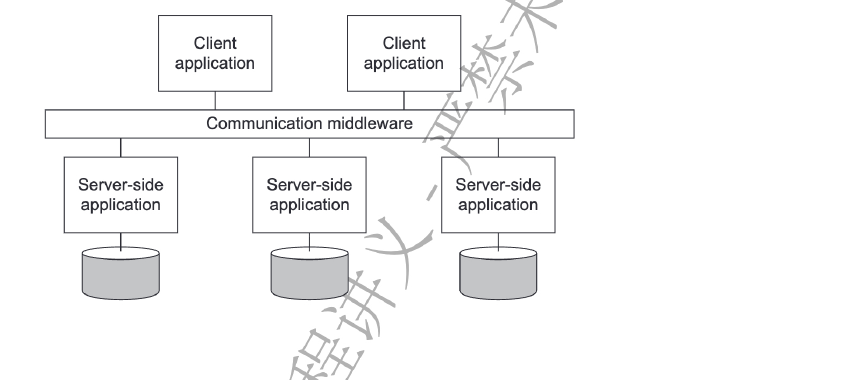
\includegraphics[width=0.68\textwidth]{figures/ch1/communication-middleware.png}
\caption{通过通信中间件连接客户端应用和服务端应用}
\end{figure}

\subsection{透明性}

\subsubsection*{透明性}

\begin{itemize}
  \item \textbf{透明性：}\blue{对用户和应用程序隐藏系统组件的物理分布性。}
  \item \textbf{理想目标：}\blue{使分布式系统使用体验接近单机系统。}
\end{itemize}

\begin{figure}[H]
\centering
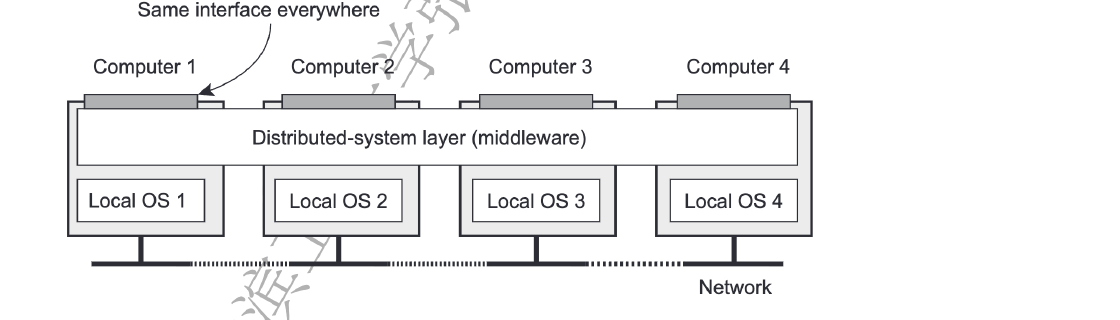
\includegraphics[width=0.78\textwidth]{figures/ch1/distributed-system-layer.png}
\caption{分布透明性的内涵}
\end{figure}

\paragraph{实现透明性：中间件}
位于 OS 与应用间的软件层，提供分布式系统共性服务。被称为：分布式系统的操作系统。典型技术：
\begin{itemize}
  \item 远程过程调用（RPC）：封装网络通信，支持同步/异步调用。
  \item 面向消息的中间件（MOM）：消息发送到逻辑联系点（发布），并转发给订阅的应用程序。
\end{itemize}

\paragraph{实现透明性：虚拟化}
\begin{figure}[H]
\centering
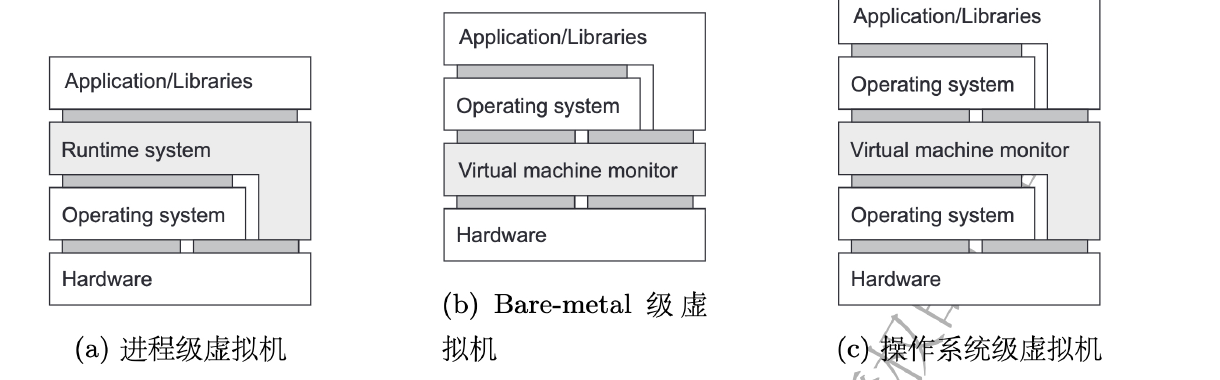
\includegraphics[width=0.88\textwidth]{figures/ch1/virtualization-types.png}
\caption{进程级、Bare-metal 级与操作系统级虚拟机}
\end{figure}

\begin{itemize}
  \item 核心优势：
  \begin{itemize}
    \item 支持计算迁移与负载均衡
    \item 故障/安全隔离
  \end{itemize}
\end{itemize}

\paragraph{透明性 $\ne$ “完全隐身”}
\begin{itemize}
  \item 追求“绝对透明”可能适得其反：系统会为“假装是单机”付出过高代价（如性能下降、复杂度飙升）。
  \item “绝对透明”可能只是个梦：
  \begin{itemize}
    \item 故障 vs. 慢
    \begin{itemize}
      \item 服务器没回消息，是崩溃了？还是卡在垃圾回收？
      \item 发微信：对方不回，是手机没电了，还是在装没看见？
    \end{itemize}
    \item 操作到底执行没？不确定！
    \begin{itemize}
      \item 服务器收到请求后刚写日志，就断电了……操作成功了吗？
      \item 网络超时重传？可能重复执行！
    \end{itemize}
  \end{itemize}
\end{itemize}

\paragraph{有时，“暴露分布性”更好}
敢说实话，反而更可靠、更高效：
\begin{itemize}
  \item 明确故障提示：“连接超时（30 秒无响应）”比“卡住不动”更友好。用户可选择：重试 / 换节点 / 稍后再试。
\end{itemize}

\paragraph{核心思想}
\blue{透明性是目标，但不是教条，平衡易用性、性能与可靠性才是关键。}

\subsection{开放性}

\subsubsection*{开放性}

\blue{系统通过标准化接口与协议支持互操作与集成。}要求：
\begin{itemize}
  \item 符合开放标准（如 HTTP, gRPC, OpenAPI）
  \item 支持跨平台应用互操作
  \item 保障应用可移植性
  \item 便于功能扩展
\end{itemize}

\subsection{可信任性}

\subsubsection*{可信任性}

\blue{可信任性（Dependability）的四大内涵：}

\begin{table}[H]
\centering
\caption{可信任性的核心要求}
\begin{tabularx}{\textwidth}{>{\raggedright\arraybackslash}p{0.34\textwidth}X}
\toprule
\textbf{要求} & \textbf{描述} \\
\midrule
\blue{可用性}（Availability） & 准备好供使用 \\
\blue{可靠性}（Reliability） & 服务交付的连续性 \\
\blue{安全性}（Safety） & 极低的灾难发生概率 \\
\blue{可维护性}（Maintainability） & 故障系统修复的难易程度 \\
\bottomrule
\end{tabularx}
\end{table}

\paragraph{故障、错误与失效}

\begin{table}[H]
\centering
\caption{故障、错误与失效}
\begin{tabularx}{\textwidth}{>{\raggedright\arraybackslash}p{0.22\textwidth}X>{\raggedright\arraybackslash}p{0.2\textwidth}}
\toprule
\textbf{术语} & \textbf{描述} & \textbf{示例} \\
\midrule
\blue{故障}（Fault） & 系统中可能导致失效的异常\textbf{源头} & 软件 Bug \\
\blue{错误}（Error） & 故障后导致的内部不正确\textbf{状态} & 内存越界 \\
\blue{失效}（Failure） & 系统对外表现出的不符合规格的\textbf{表现} & 停止服务 \\
\bottomrule
\end{tabularx}
\end{table}

\paragraph{术语：处理缺陷}
\begin{table}[H]
\centering
\caption{处理缺陷的术语}
\begin{tabularx}{\textwidth}{>{\raggedright\arraybackslash}p{0.24\textwidth}X>{\raggedright\arraybackslash}p{0.18\textwidth}}
\toprule
\textbf{术语} & \textbf{描述} & \textbf{示例} \\
\midrule
\blue{预防}（Prevention） & 防止故障的发生 & 代码审查 \\
\blue{容错}（Fault tolerance） & 故障（Fault）发生系统依然可正常运行的能力 & 冗余、副本 \\
\blue{消除}（Elimination） & 减少故障的存在、数量或严重性 & 补丁更新 \\
\blue{预测}（Prediction） & 估计故障的未来发生率和后果 & 压力测试 \\
\bottomrule
\end{tabularx}
\end{table}

\subsection{安全性}

\subsubsection*{安全性}

\blue{安全是可靠性的必要前提。}核心需求：
\begin{itemize}
  \item \blue{保密性}（Confidentiality）：信息仅向授权方披露
  \item \blue{完整性}（Integrity）：确保对系统资产的更改只能以授权方式进行
  \item \blue{可用性}（Availability）：防止服务拒绝（与可靠性交叉）
\end{itemize}

\paragraph{安全性机制}
授权（Authorization），认证（Authentication），信任（Trust）
\begin{itemize}
  \item \blue{认证：}验证声称的身份的正确性
  \item \blue{授权：}确定已认证实体的访问权限
  \item \blue{信任：}一个实体可以确信另一个实体将根据特定期望执行特定操作
\end{itemize}

\subsection{可扩展性}

\subsubsection*{可扩展性}

\begin{itemize}
  \item \blue{规模可扩展性}（Size scalability）：支持用户/节点/资源数量增长
  \item \blue{地理可扩展性}（Geographic scalability）：跨地域部署与低延迟访问
  \item \blue{管理可扩展性}（Administrative scalability）：支持多自治域策略协同
  \item 挑战：地理与管理可扩展性仍是主要瓶颈。
\end{itemize}

\paragraph{地理可扩展性的难点}
\begin{itemize}
  \item 高延迟破坏同步交互模型（如 RPC 超时）
  \item WAN 链路丢包率高不可靠，影响流媒体等实时应用
  \item 广播不可行，需专用命名/目录服务（如 DNS, LDAP）
  \item 时钟同步精度不完美，影响事件排序
\end{itemize}

\paragraph{管理可扩展性的难点}
\begin{itemize}
  \item 本质：\blue{关于使用、管理和安全的策略冲突}
  \item 模范示例：部分 P2P 系统（如 BitTorrent, 早期 Skype）依赖用户自发协作或严格的分布式协议，实现管理可扩展。
\end{itemize}

\paragraph{扩展技术 I：应对通信延迟}
\begin{itemize}
  \item 异步通信与非阻塞 I/O
  \item 回调（Callback）或 Future/Promise 模式
  \item 限制：需应用逻辑支持异步模型
\end{itemize}

\paragraph{扩展技术 II：云边端协同应对服务器和通信负载}
\begin{itemize}
  \item 将计算卸载至客户端或边缘节点
  \item 减轻服务器负载，提升响应速度
\end{itemize}

\begin{figure}[H]
\centering
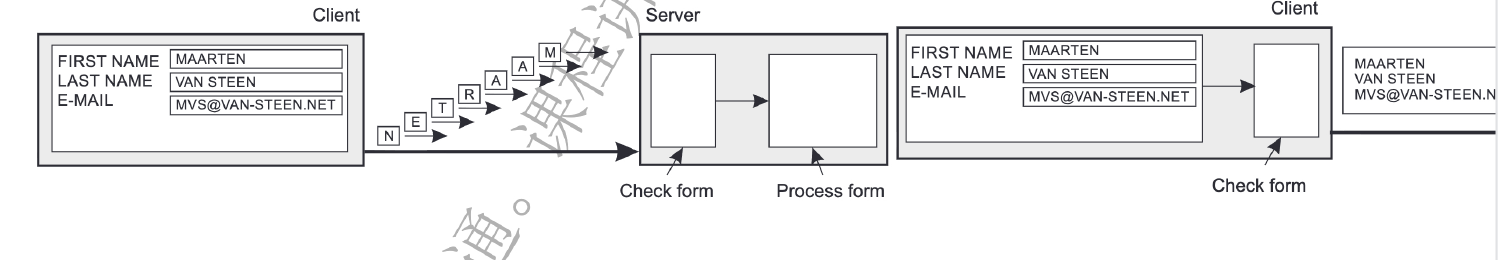
\includegraphics[width=\textwidth]{figures/ch1/client-server-form.png}
\caption{客户端与服务器协同处理表单}
\end{figure}

\paragraph{扩展技术 III：复制与缓存}
\begin{itemize}
  \item 复制：强一致性副本（如数据库主从）
  \item 缓存：弱一致性副本（如 CDN、浏览器缓存）
  \item 典型应用：
  \begin{itemize}
    \item 镜像站点
    \item Web 代理缓存
    \item 文件缓存（在服务器和客户端）
  \end{itemize}
\end{itemize}

\paragraph{复制的问题}
\begin{itemize}
  \item 有多个副本（缓存或复制）会导致不一致：修改一个副本会使该副本与其他副本不同。
  \item 始终保持副本与主副本完全同步需要全局同步每个修改，如何实现并提高效率？
\end{itemize}

\section*{结束语}
汇报完毕，欢迎同学们批评指教！本次课大致对应课程教材第一章。
